\pagestyle{appendix}
\appendix
\section*{Appendices}
\addcontentsline{toc}{section}{Appendices}
\renewcommand{\thesubsection}{\Alph{subsection}}

\subsection{Additional Graphs}

\begin{figure*}[h!]
    \centering
    \begin{subfigure}[b]{0.4\textwidth}
        \centering
        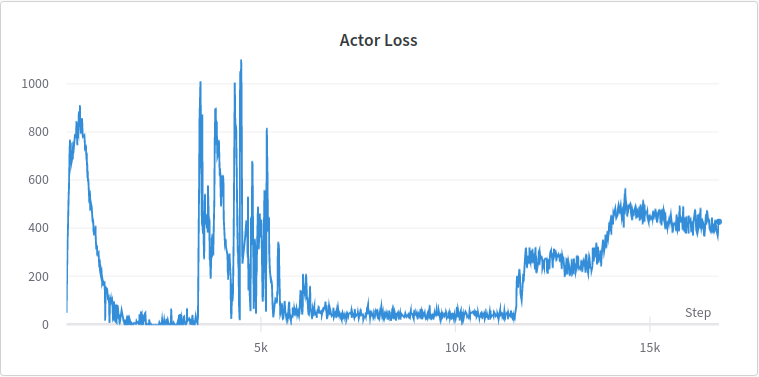
\includegraphics[width=\textwidth]{images/FRAL}
        \caption[Network2]%
        {{\small Actor Loss}}    
        \label{fig:mean and std of net14}
    \end{subfigure}
    \hfill
    \begin{subfigure}[b]{0.4\textwidth}  
        \centering 
        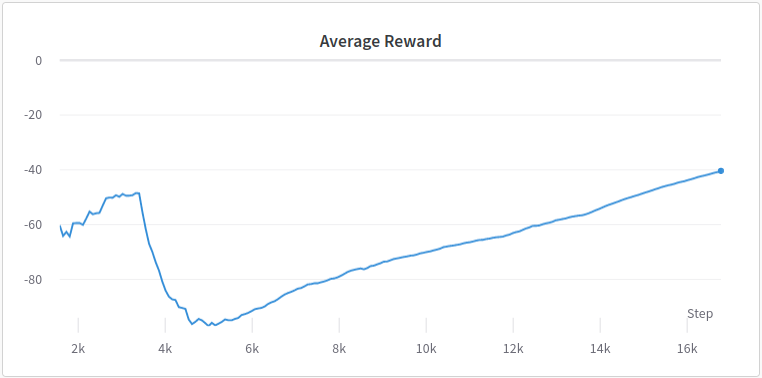
\includegraphics[width=\textwidth]{images/FRAR}
        \caption[]%
        {{\small Average Reward}}    
        \label{fig:mean and std of net24}
    \end{subfigure}
    \vskip\baselineskip
    \begin{subfigure}[b]{0.4\textwidth}   
        \centering 
        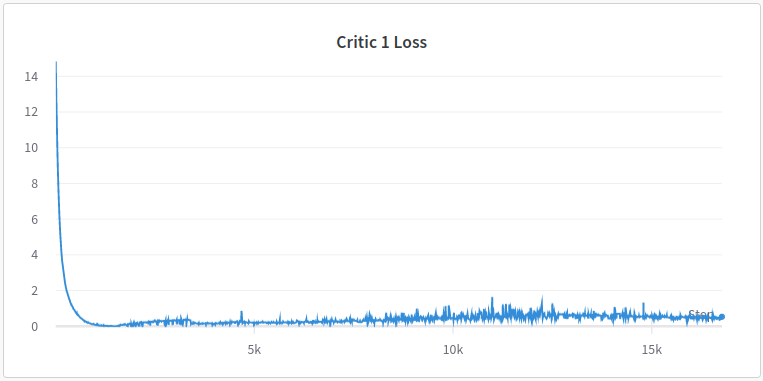
\includegraphics[width=\textwidth]{images/FRC1L.png}
        \caption[]%
        {{\small Critic 1 Loss}}    
        \label{fig:mean and std of net34}
    \end{subfigure}
    \hfill
    \begin{subfigure}[b]{0.4\textwidth}   
        \centering 
        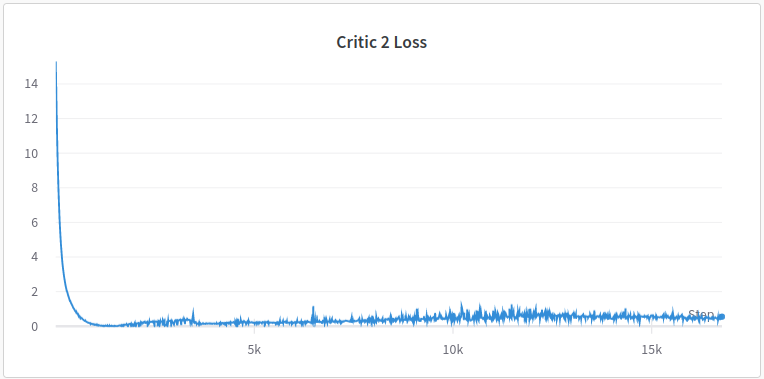
\includegraphics[width=\textwidth]{images/FRC2L.png}
        \caption[]%
        {{\small Critic 2 Loss}}    
        \label{fig:mean and std of net44}
    \end{subfigure}
    \caption[ Rewards and Loss Plots for the Fetch Reach Environment. ]
    {\small Rewards and Loss Plots for the Fetch Reach Environment.} 
    \label{fig:mean and std of nets}
\end{figure*}

\begin{figure*}[h!]
    \centering
    \begin{subfigure}[b]{0.4\textwidth}
        \centering
        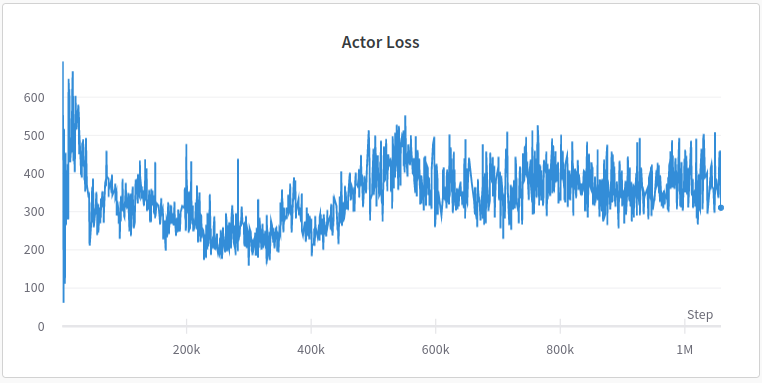
\includegraphics[width=\textwidth]{images/FPAL}
        \caption[Network2]%
        {{\small Actor Loss}}    
        \label{fig:mean and std of net14}
    \end{subfigure}
    \hfill
    \begin{subfigure}[b]{0.4\textwidth}  
        \centering 
        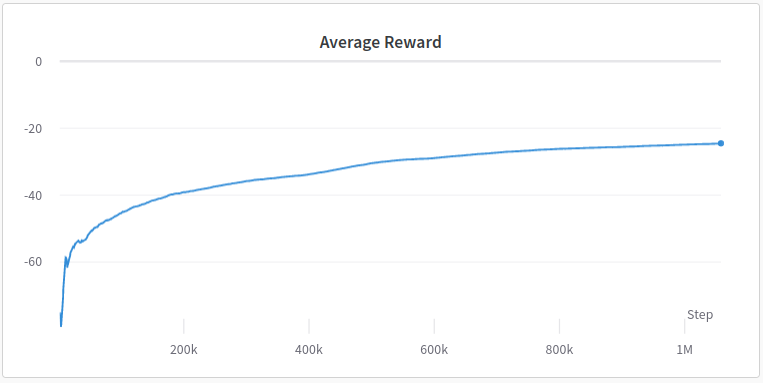
\includegraphics[width=\textwidth]{images/FPAR}
        \caption[]%
        {{\small Average Reward}}    
        \label{fig:mean and std of net24}
    \end{subfigure}
    \vskip\baselineskip
    \begin{subfigure}[b]{0.4\textwidth}   
        \centering 
        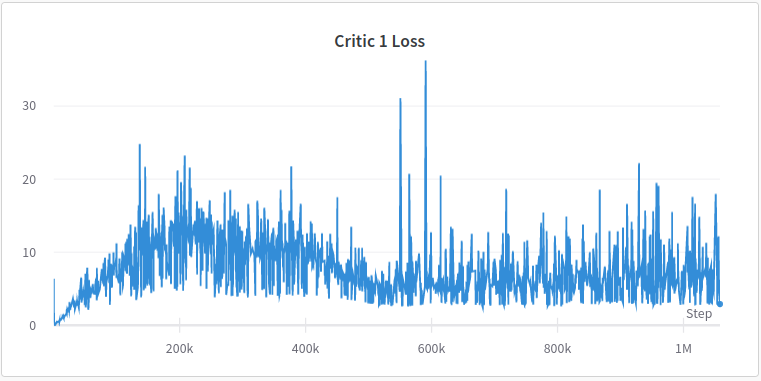
\includegraphics[width=\textwidth]{images/FPC1L.png}
        \caption[]%
        {{\small Critic 1 Loss}}    
        \label{fig:mean and std of net34}
    \end{subfigure}
    \hfill
    \begin{subfigure}[b]{0.4\textwidth}   
        \centering 
        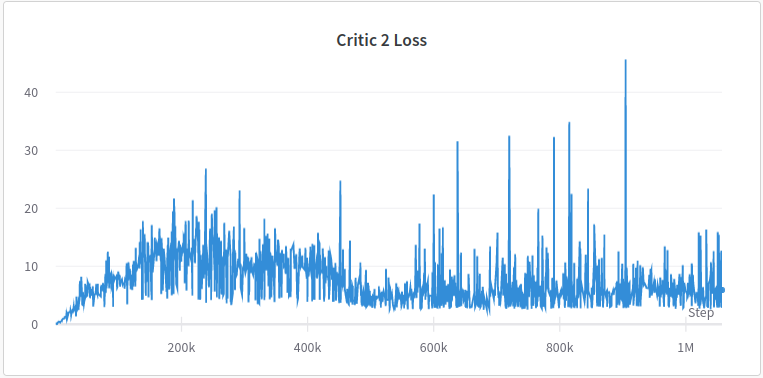
\includegraphics[width=\textwidth]{images/FPC2L.png}
        \caption[]%
        {{\small Critic 2 Loss}}    
        \label{fig:mean and std of net44}
    \end{subfigure}
    \caption[ Rewards and Loss Plots for the Fetch Push Environment. ]
    {\small Rewards and Loss Plots for the Fetch Push Environment.} 
    \label{fig:mean and std of nets}
\end{figure*}

\begin{figure*}[h!]
    \centering
    \begin{subfigure}[b]{0.475\textwidth}
        \centering
        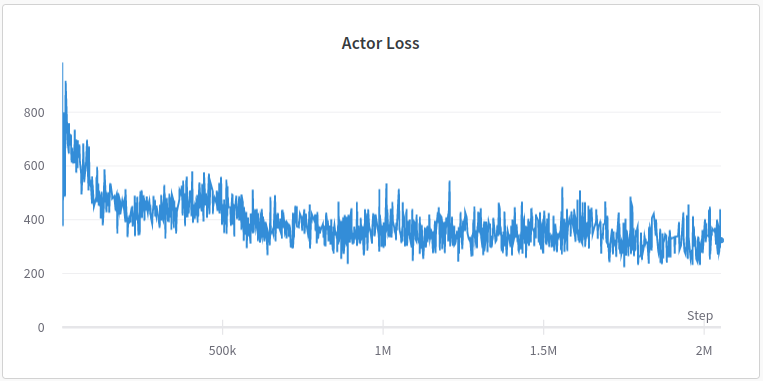
\includegraphics[width=\textwidth]{images/FSAL}
        \caption[Network2]%
        {{\small Actor Loss}}    
        \label{fig:mean and std of net14}
    \end{subfigure}
    \hfill
    \begin{subfigure}[b]{0.475\textwidth}  
        \centering 
        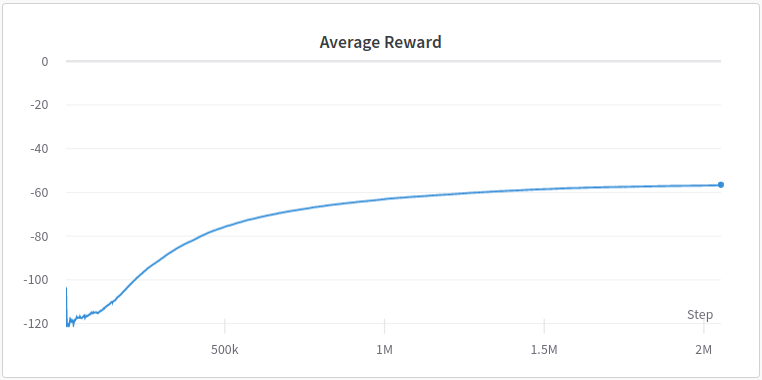
\includegraphics[width=\textwidth]{images/FSAR}
        \caption[]%
        {{\small Average Reward}}    
        \label{fig:mean and std of net24}
    \end{subfigure}
    \vskip\baselineskip
    \begin{subfigure}[b]{0.475\textwidth}   
        \centering 
        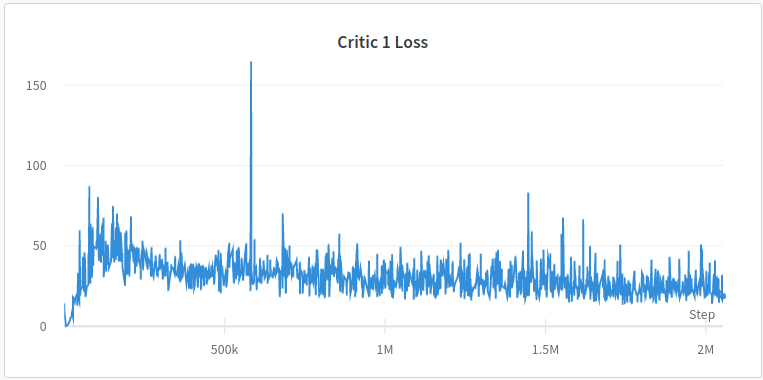
\includegraphics[width=\textwidth]{images/FSC1L.png}
        \caption[]%
        {{\small Critic 1 Loss}}    
        \label{fig:mean and std of net34}
    \end{subfigure}
    \hfill
    \begin{subfigure}[b]{0.475\textwidth}   
        \centering 
        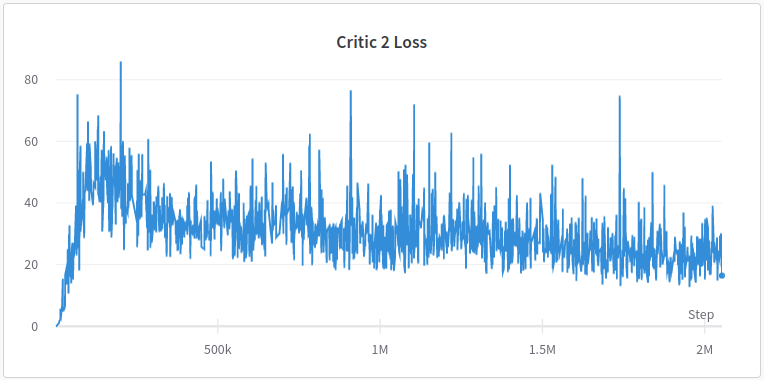
\includegraphics[width=\textwidth]{images/FSC2L.png}
        \caption[]%
        {{\small Critic 2 Loss}}    
        \label{fig:mean and std of net44}
    \end{subfigure}
    \caption[ Rewards and Loss Plots for the Fetch Slide Environment. ]
    {\small Rewards and Loss Plots for the Fetch Slide Environment.} 
    \label{fig:mean and std of nets}
\end{figure*}

\begin{figure*}[h!]
    \centering
    \begin{subfigure}[b]{0.475\textwidth}
        \centering
        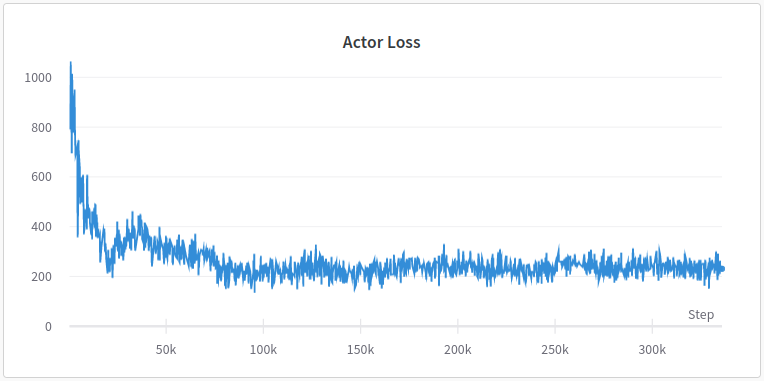
\includegraphics[width=\textwidth]{images/FPAPAAL.png}
        \caption[Network2]%
        {{\small Actor Loss}}    
        \label{fig:mean and std of net14}
    \end{subfigure}
    \vskip\baselineskip
    \begin{subfigure}[b]{0.475\textwidth}   
        \centering 
        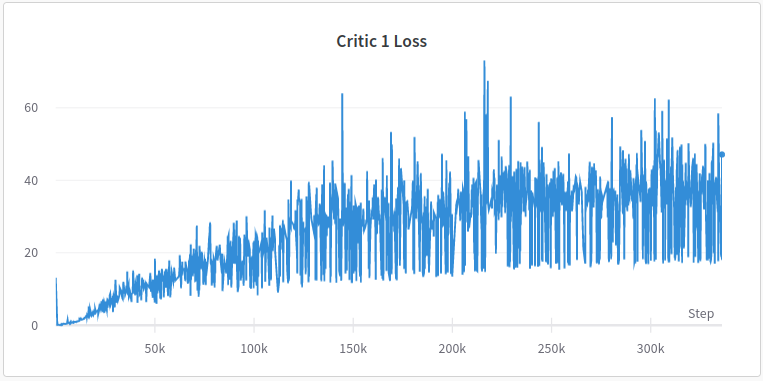
\includegraphics[width=\textwidth]{images/FPAPAC1L.png}
        \caption[]%
        {{\small Critic 1 Loss}}    
        \label{fig:mean and std of net34}
    \end{subfigure}
    \hfill
    \begin{subfigure}[b]{0.475\textwidth}   
        \centering 
        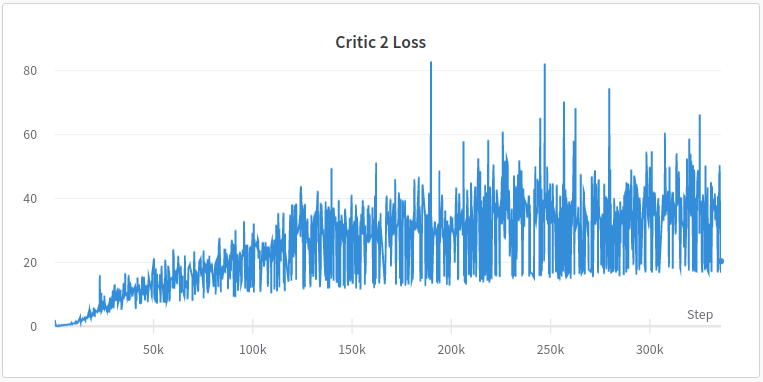
\includegraphics[width=\textwidth]{images/FPAPAC2L.png}
        \caption[]%
        {{\small Critic 2 Loss}}    
        \label{fig:mean and std of net44}
    \end{subfigure}
    \caption[ Rewards and Loss Plots for the Fetch Pick and Place Environment with Agent Demonstrator. ]
    {\small Rewards and Loss Plots for the Fetch Pick and Place Environment with Agent Demonstrator.} 
    \label{fig:mean and std of nets}
\end{figure*}

\begin{figure*}[h!]
    \centering
    \begin{subfigure}[b]{0.475\textwidth}
        \centering
        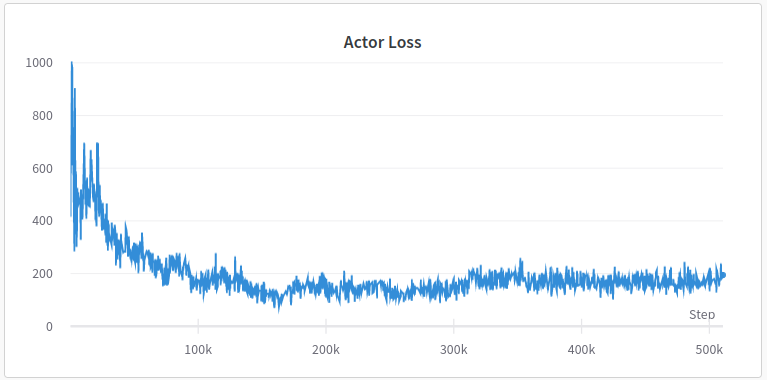
\includegraphics[width=\textwidth]{images/FPAPSAL.png}
        \caption[Network2]%
        {{\small Actor Loss}}    
        \label{fig:mean and std of net14}
    \end{subfigure}
    \vskip\baselineskip
    \begin{subfigure}[b]{0.475\textwidth}   
        \centering 
        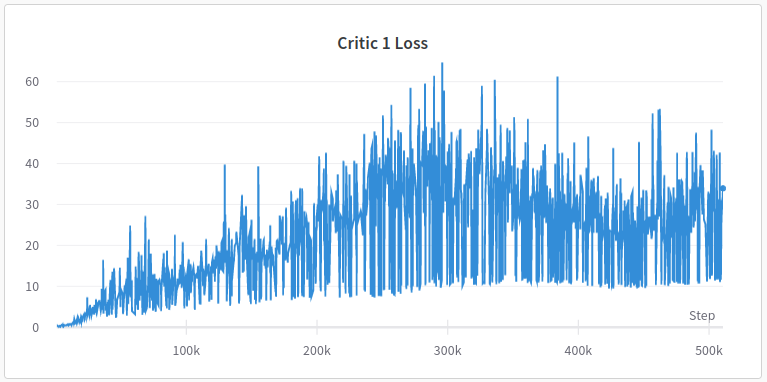
\includegraphics[width=\textwidth]{images/FPAPSC1L.png}
        \caption[]%
        {{\small Critic 1 Loss}}    
        \label{fig:mean and std of net34}
    \end{subfigure}
    \hfill
    \begin{subfigure}[b]{0.475\textwidth}   
        \centering 
        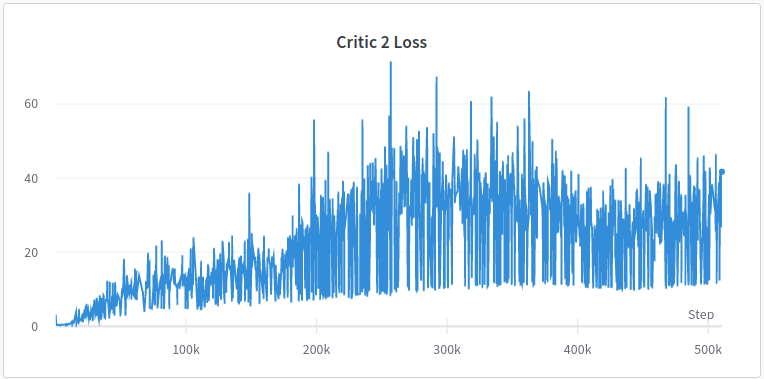
\includegraphics[width=\textwidth]{images/FPAPSC2L.png}
        \caption[]%
        {{\small Critic 2 Loss}}    
        \label{fig:mean and std of net44}
    \end{subfigure}
    \caption[ Rewards and Loss Plots for the Fetch Pick and Place Environment with Script Demonstrator. ]
    {\small Rewards and Loss Plots for the Fetch Pick and Place Environment with Script Demonstrator.} 
    \label{fig:mean and std of nets}
\end{figure*}
